% ~ 8-10 pages
\chapter{Decay Mode Classification of Hadronic Tau Lepton Decays}
\label{sec:decaymode}

In this chapter the sequence learning techniques developed for
tau-identification are applied to the problem of decay mode classification of
hadronic tau lepton decays. In the following the decay modes containing one
charged hadron~$h^\pm$ with one~$h^\pm \pi^0$ or more than one neutral
pion~$h^\pm \geq 2\pi^0$ as well as three charged hadrons without
neutrals~$3h^\pm$ or at least one neutral pion~$3h^\pm \geq 1\pi^0$ shall be
discriminated. The hadron~$h^\pm$ includes charged pions as well as kaons while
decays over intermediate~$\text{K}^0$ are omitted. These five decay modes make
up the majority of hadronic tau decays (approx.\ \SI{92}{\percent}). Neural
networks naturally extend from binary to multi-class classification problems
making them well-suited for the discrimination of the hadronic decay modes.

At first a quick overview of the \emph{Tau Particle Flow}-algorithm is given,
which is used to reconstruct neutral and charged decay products. Subsequently a
neural network is developed that uses the reconstructed decay products to
classify the decay mode into one of five categories. Finally the network is
extended by including additional information from conversion tracks, cluster
moments and shot information. In the following the notation established in
Ref.~\cite{atlas:taurec:decaymodes} will be adopted.

\todo[inline]{Signature of the decay modes (Could be moved to
  \textit{Theoretical Background})}

\todo[inline]{Plot some discriminating variables?}

\section{Tau Particle Flow}
\label{sec:tau_pflow}

The \emph{Tau Particle Flow}-algorithm is a specialised particle flow algorithm
for reconstruction of charged and neutral constituents in hadronic tau decays
with visible transverse momenta of up to \SI{100}{\giga\electronvolt}. It aims
to improve reconstruction of individual particles by optimally combining the
information in several subdetector-systems. The reconstructed objects, called
charged or neutral \emph{particle flow objects}~(PFOs), can be used to classify
the hadronic decay modes and for improving the energy resolution of the
reconstructed hadronic tau decay by employing a decay mode specific calibration.
The following description of the algorithm is based on
Ref.~\cite{atlas:taurec:decaymodes} including recent changes to the reconstruction
algorithms.

Charged PFOs are reconstructed from tracks classified as \emph{charged}
according to the track classification. The charge and transverse momentum of the
reconstructed PFO is determined from the measurement in the tracking system,
which has superior energy resolution for charged pions with
$p_\text{T} < \SI{100}{\giga\electronvolt}$ compared to a calorimeter-based
measurement~\cite{atlas:taurec:decaymodes}. The $\pi^\pm$-mass hypothesis is
used to calculate the energy of the PFO.
% Charged hadrons initiate extensive
% hadronic showers depositing most of their energy in the hadronic calorimeters
% (incl.\ EM3) \todo{Motivation for this sentence?}.

Neutral pions often deposit their energy in a single cluster in the EM
calorimeter (Presampler, EM1/EM2) caused by two collimated photons from the
$\pi^0$~decay. Therefore neutral PFOs are reconstructed by clustering all cells
in the electromagnetic part of the calorimeter within the~$\Delta R < 0.4$ cone
about the tau axis \todo{Check instead of core-region?}. If a cluster is in the
proximity of a charged PFO then the energy deposition of the charged hadron in
the EM calorimeter has to be separated from the neutral pion energy. The energy
$E_{h^\pm}^{\text{EM}}$ that needs to be subtracted to remove the contribution
of the charged hadron is estimated by
\begin{align*}
  E_{h^\pm}^{\text{EM}} = E_{h^\pm}^{\text{track}} - E_{h^\pm}^{\text{HAD}} \eqcomma
\end{align*}
where $E_{h^\pm}^{\text{track}}$ is the energy of the charged PFO measured in
the tracking system and $E_{h^\pm}^{\text{HAD}}$ the energy of the charged PFO
deposited in the hadronic part of the calorimeter. $E_{h^\pm}^{\text{HAD}}$ is
calculated by matching clustered energy deposits in the HCAL to the closest
track of a charged PFO. The contribution of the charged hadron in the EM
calorimeter~$E_{h^\pm}^{\text{EM}}$ is subtracted from the closest neutral PFO
cluster if the angular distance between cluster and extrapolated track is
smaller than~$\Delta R < 0.04$. \todo{Zero mass hypothesis for neutrals?}
Neutral PFOs can often be reconstructed from an incomplete subtraction of the
charged hadron energy deposition in the EM calorimeter or by pile-up. For decay
mode classification it is necessary to identify the neutral pions in all
reconstructed neutral PFOs of the tau decay. The identification exploits the
difference in shower shape of hadronic showers initiated by charged hadrons and
compact showers from photons of the $\pi^0$ decay using multivariate methods.

The number of identified neutral pions can be used for a preliminary
classification of the decay mode. The following sections will be concerned with
combining reconstructed PFOs in neural networks to achieve better classification
power. Decay mode classification employing the \emph{Tau Particle
  Flow}-algorithm is optimised for operation in the low-momentum regime due to
the decreasing momentum resolution in the tracking system as well as the
additional boost of the tau decay products leading to merging of
$\pi^0$-clusters. Therefore the main focus is on the classification of hadronic
tau lepton decays with visible transverse
momenta~$p_\text{T} < \SI{100}{\giga\electronvolt}$ but prospects of a
classification algorithm usable over an extended momentum range are also given.

\section{Classification with Tau Particle Flow and Recurrent Neural Networks}
\label{sec:pfo_general}

The charged and neutral PFOs reconstructed with the \emph{Tau Particle
  Flow}-algorithm contain information about the daughter particles of the tau
decay and can be used for decay mode classification. Properties of charged and
neutral PFOs are combined in recurrent neural networks to perform multi-class
classification. Mainly kinematic information, e.g.\ the transverse momentum and
angular deviation from the tau axis, is used to describe each PFO. Moreover the
$\pi^0$-likeness in form of the neutral pion identification score is included in
the classification to be able to discriminate between neutral PFOs originating
from a neutral pion and remnants of the subtraction or pile-up.

\begin{figure}[htb]
  \centering
  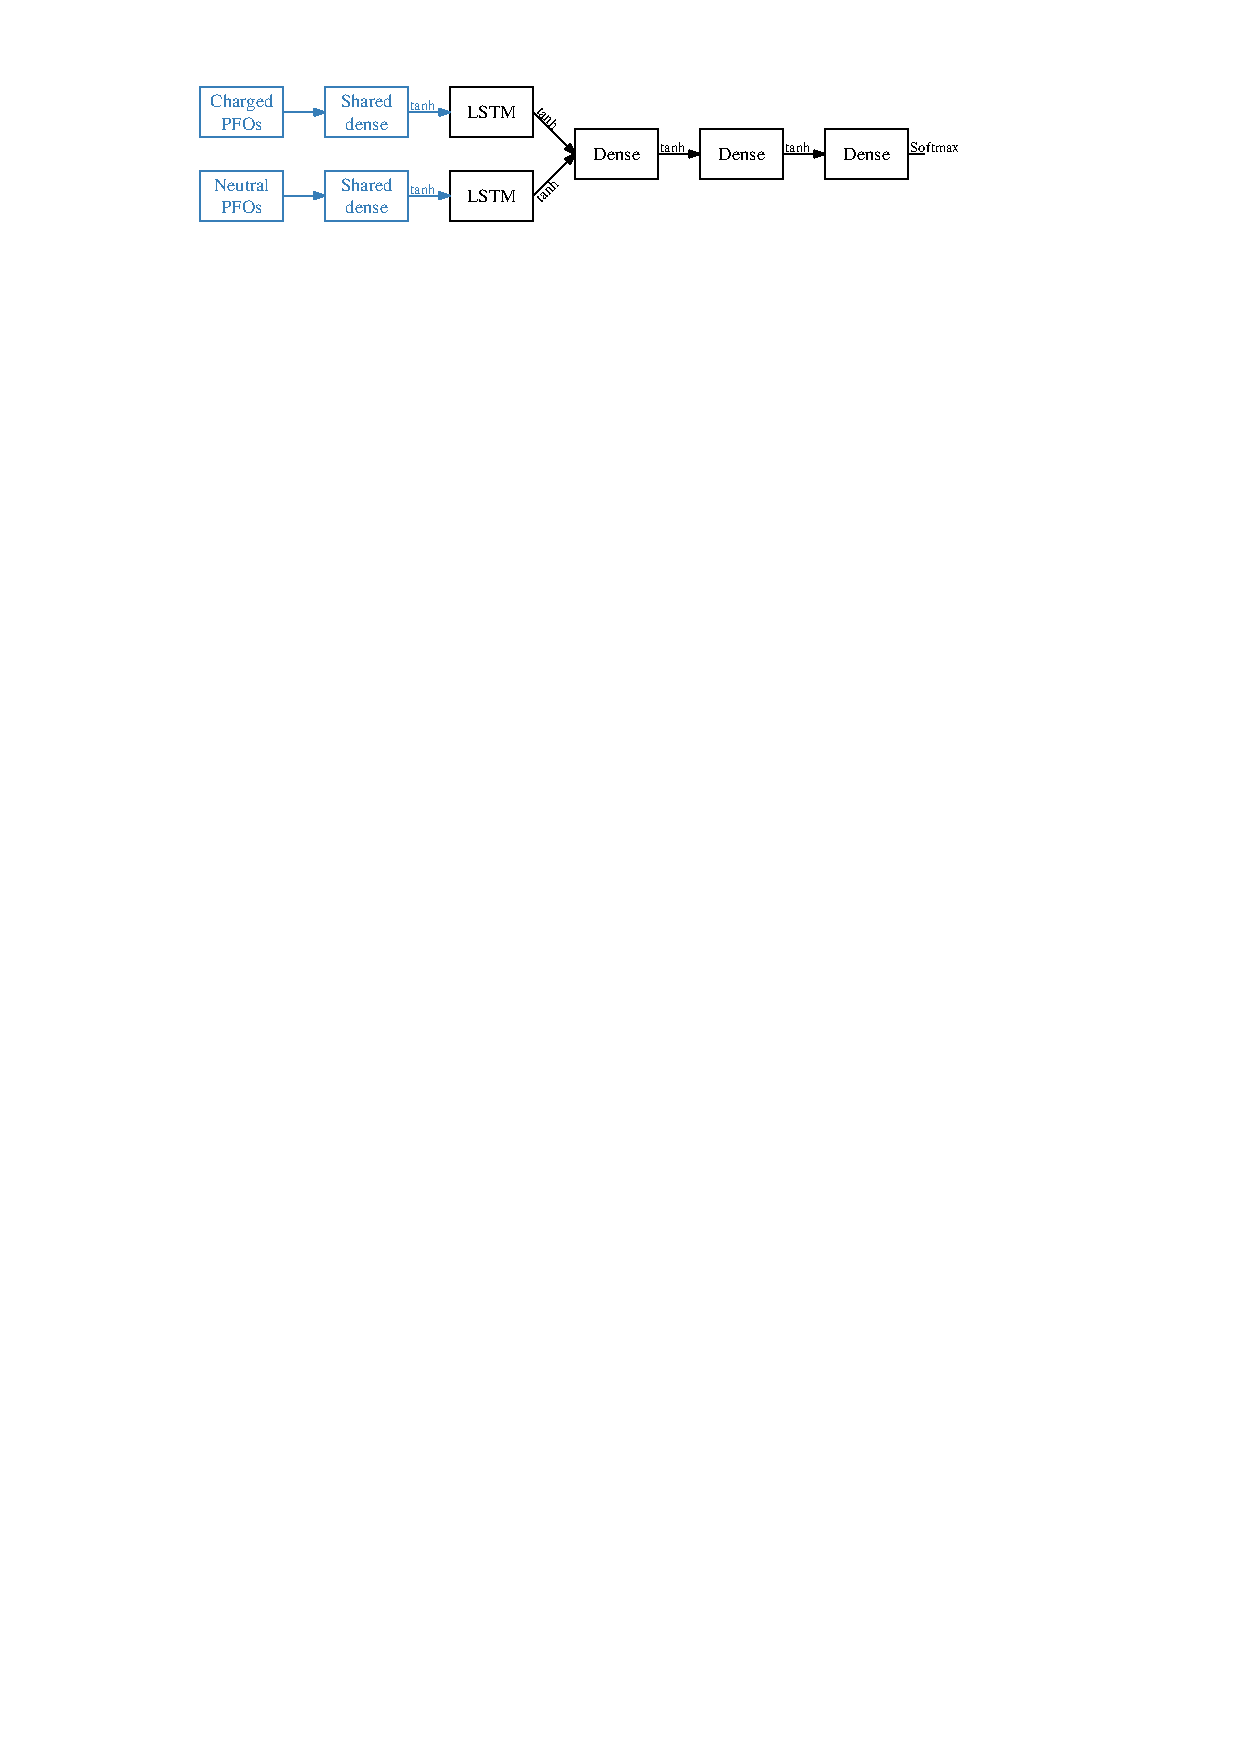
\includegraphics{./figures/decay_mode_classification/baseline_architecture.pdf}
  \caption{Architecture of the baseline model operating on sequences of charged
    and neutral PFOs. The activation function is denoted after each layer.
    Layers operating on sequential inputs are highlighted in blue.}
  \label{fig:pfo_rnn_baseline_arch}
\end{figure}

The network architecture used for the decay mode classification is shown in
Figure~\ref{fig:pfo_rnn_baseline_arch} and is similar to the networks used for
tau-identification in the previous chapter. The inputs of the network are split
into two branches each accepting a number of charged and neutral PFOs. A shared
dense layer applies an affine transformation to the input variables of each PFO.
Afterwards the transformed sequences are fed into the recurrent layer returning
a single vector of activations. The activations of both branches are
concatenated and passed through a network containing three dense layers. The
final dense layer has five units equal to the number of decay modes to classify.
Application of the Softmax activation function on the final layer ensures that
the output activations can be interpreted as mode probabilities.

\subsection{Baseline Model}
\label{sec:pfo_baseline}

For training and evaluation of the model a sample of the
process~$\gamma^* \rightarrow \tau \tau \, \text{(hadr.)}$ is used (cf.\
Section~\ref{sec:bdt_eventsim}). Compared to the dataset used for the
tau-identification studies, it features an updated tuning of the default decay
mode classification and an increase in the number of simulated events by
\SI{50}{\percent}. The sample identifier is given in
Appendix~\ref{app:mc16a_taus}.

\begin{table}[htb]
  \centering
  \begin{tabular}{
  l
  S[table-format=2.2(2)]
  S[table-format=2.1(2)]
  S[table-format=2.1, round-mode=places, round-precision=1]
  S[table-format=2.1, round-mode=places, round-precision=1]
  }
  \toprule
  {Mode} & {$\mathcal{B}$ / \si{\percent}} & {$f_\text{BR}$ / \si{\percent}} & {$f_\text{reco}$ / \si{\percent}} & { $f_\text{reco+ID}$ / \si{\percent}} \\
  \midrule
  $h^\pm$ & 11.51 +- 0.05 & 18.3 +- 0.1 & 17.552988 & 21.365416 \\
  $h^\pm \pi^0$ & 25.93 +- 0.09 & 41.3 +- 0.2 & 41.854581 & 44.779216 \\
  $h^\pm \geq 2 \pi^0$ & 10.81 +- 0.09 & 17.2 +- 0.2 & 18.663134 & 15.775690 \\
  $3 h^\pm$ & 9.43 +- 0.05 & 15.1 +- 0.1 & 14.200414 & 13.315444 \\
  $3 h^\pm \geq 1 \pi^0$ & 5.09 +- 0.05 & 8.1 +- 0.1 & 7.728881 & 4.764232 \\
  \bottomrule
\end{tabular}

%%% Local Variables:
%%% mode: latex
%%% TeX-master: "../mythesis"
%%% End:

  \caption{Mode reconstruction efficiencies. $h^\pm$ can be pion or kaon.
    Intermediate decays via neutral kaons are excluded. Branching fraction
    $\mathcal{B}$; Mode fractions of reconstructed taus passing preselection
    $f_\text{reco}$; Mode fraction of taus also passing medium tau id.
    $f_\text{BR}$ fraction assuming fully efficient reconstruction.}
  \label{tab:mode_reco_eff}
  \todo[inline]{What should be in this table?}
\end{table}

In addition to the baseline selection given in Section~\ref{sec:bdt_eventsim},
the visible transverse momentum of the hadronic tau decay is required to be less
than \SI{100}{\giga\electronvolt} at reconstruction and generator-level.
Moreover, only taus with the generated decay mode being one of $h^\pm$,
$h^\pm \pi^0$, $h^\pm \geq 2\pi^0$, $3h^\pm$ or $3h^\pm \geq 1\pi^0$ and
omitting decays containing intermediate~\smash{$\text{K}^0$} are used. The mode
composition of the sample after applying this preselection is summarised in
Table~\ref{tab:mode_reco_eff}.

The discrimination of the decay modes utilises kinematic quantities of the
reconstructed tau decay as well as the charged and neutral particle flow
objects. The neutral and charged PFO variables are summarised in the following:
\begin{description}
\item[Kinematic quantities of the reconstructed tau decay:] The visible
  transverse momentum~$p_\text{T}^\tau$ and the angular
  direction~$(\varphi_\tau, \eta_\tau)$ of the reconstructed tau-axis. The
  momentum is calibrated at LC-scale without applying a tau-specific energy
  calibration.

\item[Kinematic quantities of charged and neutral PFOs:] The reconstructed
  transverse momentum $p_\text{T}^\text{PFO}$ and the signed angular distances
  to the reconstructed tau-axis in transverse~$\Delta\varphi$ and longitudinal
  direction~$\Delta\eta \coloneqq \eta_\text{PFO} - \eta_\tau$. The transverse
  angular distance~$\Delta\varphi$ is defined analogously to the longitudinal
  case but also accounting for the periodicity in the azimuthal angle~$\varphi$.
  Angular deviations from the tau-axis are used to ensure that coordinates are
  comparable between different tau candidates.
\end{description}
For neutral PFOs the set of variables is extended to allow for the
identification of clusters originating from neutral pions. In addition to the
kinematic quantities the following variables are used:
\begin{description}
\item[$\pi^0$-identification score $S_\text{BDT}^{\pi^0}$:] BDT-based
  discriminant combining shower shape information in the electromagnetic part of
  the calorimeter to identify neutral PFOs originating from photons of the
  $\pi^0$ decay~\cite{atlas:taurec:decaymodes}.

\item[Number of shots $N_\text{shots}$:] Number of shots (cf.\
  Section~\ref{sec:shot_reco}) associated with a neutral PFO cluster. Shots are
  associated with a cluster if it contains the seed cell of the shot and the
  cluster fulfils $E_\text{T} > \SI{500}{\mega\electronvolt}$ and is within
  $\Delta R < 0.4$ to the tau axis. In cases where the cell is shared between
  multiple clusters, it is associated to the cluster to which the seed cell
  contributes with the largest weight~\cite{athena}.

  The fine segmentation of the strip layer in the EM calorimeter is used to
  count local energy maxima created by individual photons, allowing in some
  cases to recover the correct number of neutrals when the energy depositions of
  two neutral pions are reconstructed as a single cluster in the calorimeter.
  Moreover, it supports the identification of neutral pions as no shot
  information is used in the current identification algorithm.
  \todo{\SI{1.5}{\percent} impact on diag.\ eff.}
\end{description}

Analogously to the RNN-based tau identification in Chapter~\ref{sec:rnn}, the
full dataset is split into a training~(\SI{50}{\percent}),
validation~(\SI{10}{\percent}) and testing sample~(\SI{40}{\percent}). The
transverse momenta of the reconstructed tau and PFOs are log-transformed and
subsequently standardised by subtracting the mean and dividing by the standard
deviation, derived from the distributions in the training sample. For the
neutral PFO specific variables~\smash{$S_\text{BDT}^{\pi^0}$} and
\smash{$N_\text{shots}$} no preprocessing is required. The remaining kinematic
variables, i.e.\ angular direction of the tau-axis and angular deviation of the
PFO, are scaled into the~$[-1, 1]$-interval.

Charged and neutral PFOs are passed in ascending transverse momentum ordering to
the shared dense layers with 24 units each. A maximum of three charged PFOs
corresponding to the \emph{charged} tracks and up to ten neutral PFOs are used.
The intermediate representations after the shared dense layers are passed into
the LSTM layers, each returning a vector of 24 activations. The activations of
both branches are merged and passed through a network of three dense layers with
48, 32 and 5 units, respectively.

For a given reconstructed tau decay the model returns one probability for each
of the five decay modes. The decay mode is classified as the mode with the
largest probability estimate according to the model. A different scheme for
determining the decay mode would be to require the largest mode probability to
exceed the second largest by a predefined margin. This would increase the purity
of the classified modes at the expense of reducing the efficiency. As this
scheme depends on the requirements of the particular analysis, the following
will focus on classification according to the highest probability.

In contrast to the decay mode classification algorithm currently in use at the
ATLAS experiment, no discrimination of 1- and 3-prong modes according to the
number of reconstructed tracks that are classified as \emph{charged} is made.
However, as each charged PFO is associated with a \emph{charged} track the
number of tracks is indirectly available to the network. The network is not
strictly required to use this information allowing migrations of reconstructed
1-track (3-track) hadronic tau decays to 3-prong (1-prong) modes. If this
behaviour is not desired then the decay mode can be classified as the mode with
the highest probability that is still compatible with the number of
reconstructed tracks. For the following studies these migrations are allowed as
the loss in classification power is small when constraining the model (cf.\
Appendix~\ref{app:mode_classification_track_constraint} for a comparison).

\begin{table}[htb]
  \centering
  \begin{tabular}{SS[table-format=2.2(2)]}%,table-space-text-post = \si{\meter}]}
  \toprule
  {$p_\text{T}$-cut / \si{\giga\electronvolt}} & {Diagonal efficiency / \si{\percent}} \\
  \midrule
  {--} & 78.43 \pm 0.06 \\
  1.0 & 78.09 \pm 0.08 \\
  1.5 & 77.95 \pm 0.04 \\
  2.0 & 77.88 \pm 0.06 \\
  2.5 & 77.54 \pm 0.04 \\
  \bottomrule
\end{tabular}

%%% Local Variables:
%%% mode: latex
%%% TeX-master: "../mythesis"
%%% End:

  \caption{Diagonal efficiency evaluated on the validation sample as a function
    of the transverse momentum threshold for neutral PFOs. The network is
    retrained for each threshold.}
  \label{tab:neut_ptcut}
\end{table}

Neutral PFOs with small transverse momenta often do not originate from neutral
pions but from other sources. Moreover, it is not understood how well they are
modelled in the simulation. Therefore neutral PFOs passed to the network (at
training and evaluation time) are required to exceed a predefined
$p_\text{T}$-threshold. The diagonal efficiency, i.e.\ the fraction of correctly
classified modes in an independent sample, is summarised in
Table~\ref{tab:neut_ptcut} for four different $p_\text{T}$-thresholds. The
classification power does not degrade when no $p_\text{T}$-cut is applied,
indicating that the model is insensitive to low momentum PFOs from sources other
than a \smash{$\pi^0$}-decay. This is expected as the network has access to the
\smash{$\pi^0$}-identification score and transverse momentum. Additionally, only
a slow decrease in diagonal efficiency is observed when increasing the
threshold. The studies in this thesis use a \SI{1.5}{\giga\electronvolt}
threshold to account for potential mismodelling but further studies are needed
to prove the necessity of this cut.

\begin{figure}[htb]
  \begin{subfigure}[t]{0.48\textwidth}
    \centering
    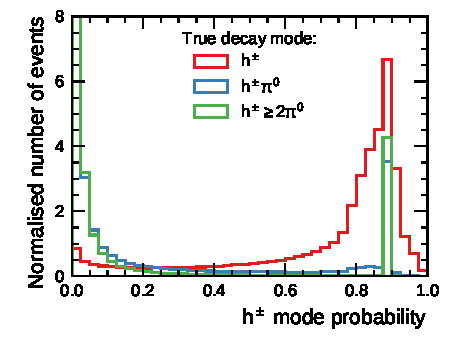
\includegraphics{./figures/decay_mode_classification/mode_proba_baseline_ptcut_1_5_only_1p/proba_1p0n.pdf}
    \vspace*{-1.6em}
    \subcaption{}
    \label{fig:1p0n_proba}
  \end{subfigure}\hfill
  \begin{subfigure}[t]{0.48\textwidth}
    \centering
    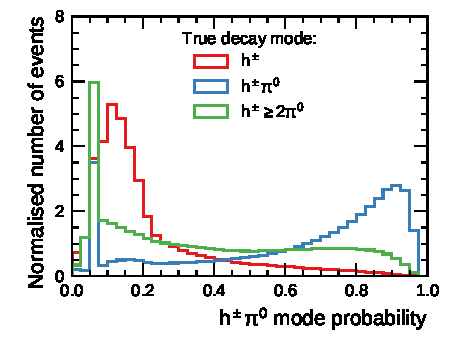
\includegraphics{./figures/decay_mode_classification/mode_proba_baseline_ptcut_1_5_only_1p/proba_1p1n.pdf}
    \vspace*{-1.6em}
    \subcaption{}
    \label{fig:1p1n_proba}
  \end{subfigure}
  \caption{Mode probabilities for the $h^\pm$ and $h^\pm \pi^0$ modes estimated
    by the RNN for a given true decay mode. Modes with three charged hadrons
    have small $h^\pm$ and $h^\pm \pi^0$ probabilities and are omitted for
    clarity.}
  \label{fig:mode_proba_ptcut}
\end{figure}

Figure~\ref{fig:mode_proba_ptcut} depicts two examples of mode probability
estimates on the testing sample. A complete set of probabilities for all five
decay modes is omitted for brevity and can be found in
Appendix~\ref{app:baseline_probabilities}. The $h^\pm$ mode probability in
Figure~\ref{fig:1p0n_proba} shows that the estimated probabilities for generated
modes containing one or more neutral pions are frequently small. Nevertheless,
when no neutral PFOs are reconstructed they can be as large as
\SI{90}{\percent}, causing decays to be falsely classified. The same feature can
be observed in Figure~\ref{fig:1p1n_proba}, where the $h^\pm \pi^0$ mode
probabilities are small. Additionally, generated 1-prong decays with more than
one neutral pion often exceed $h^\pm \pi^0$ probabilities of \SI{50}{\percent}
leading to significant migrations of true $h^\pm \geq 2 \pi^0$ to the
$h^\pm \pi^0$ decay mode.

\begin{figure}[tb]
  \begin{subfigure}[t]{0.48\textwidth}
    \centering
    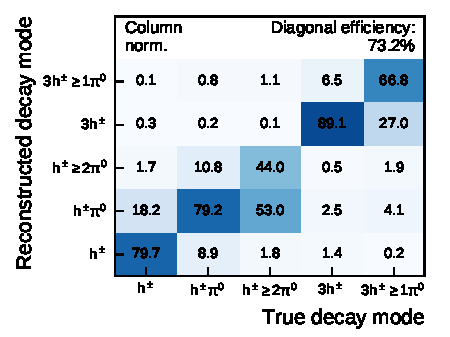
\includegraphics{./figures/decay_mode_classification/mig_mat_pantau.pdf}
    \subcaption{ATLAS default algorithm}
  \end{subfigure}\hfill
  \begin{subfigure}[t]{0.48\textwidth}
    \centering
    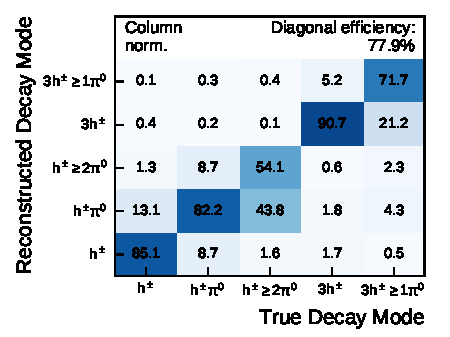
\includegraphics{./figures/decay_mode_classification/mig_mat_baseline_ptcut_1_5.pdf}
    \subcaption{RNN with neutral PFO $p_{\text{T}}$-cut of
      \SI{1.5}{\GeV}}
  \end{subfigure}
  \caption{Migration matrices showing the migration probabilities of the true
    decay modes to the reconstructed modes in \si{\percent}. Evaluation on the
    independent testing sample. Statistical fluctuations due to limited sample
    size can be neglected.}
  \label{fig:migmat_comparison_baseline_15cut}
\end{figure}

The migration probability of generated decay modes to a given reconstructed mode
can be summarised in the so called \emph{migration matrix}.
Figure~\ref{fig:migmat_comparison_baseline_15cut} shows migration matrices of
the ATLAS default algorithm~\cite{atlas:taurec:decaymodes} and the RNN-based
decay mode classification. The diagonal entries give the efficiencies to
correctly reconstruct the corresponding decay mode while the off-diagonal
measures the migration probability between modes. The diagonal efficiency can
also be interpreted as the mean of the diagonal entries of this matrix weighted
by the reconstructed mode fractions (cf.\ Table~\ref{tab:mode_reco_eff}). The
individual efficiencies and migration probabilities in the matrix can vary
between different trainings of the network as a decrease in efficiency in one
mode can be compensated by an improvement in another. Nevertheless, the diagonal
efficiency is a stable metric between different trainings and is used as a
figure of merit for subsequent investigations.

\begin{figure}[tb]
  \begin{subfigure}[t]{0.48\textwidth}
    \centering
    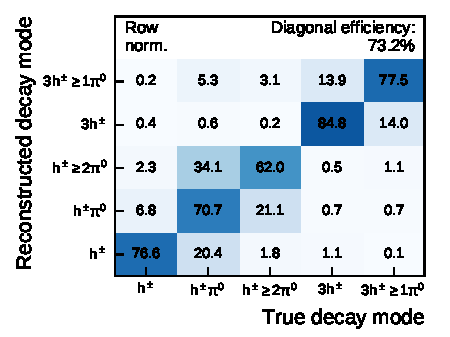
\includegraphics{./figures/decay_mode_classification/comp_mat_pantau.pdf}
    \subcaption{ATLAS default algorithm: \emph{PanTau}}
  \end{subfigure}\hfill
  \begin{subfigure}[t]{0.48\textwidth}
    \centering
    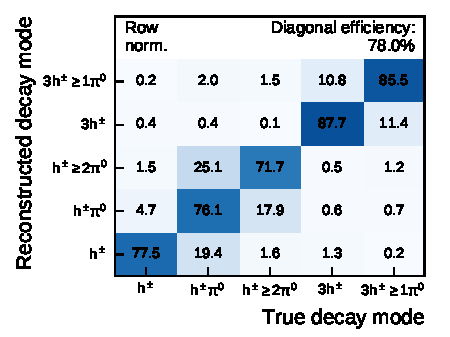
\includegraphics{./figures/decay_mode_classification/comp_mat_baseline_ptcut_1_5.pdf}
    \subcaption{RNN with neutral PFO $p_{\text{T}}$-cut of
      \SI{1.5}{\giga\electronvolt}}
  \end{subfigure}
  \caption{Purity matrices showing the fractional composition of the
    reconstructed decay modes in \si{\percent}. Evaluation on the independent
    testing sample. Statistical fluctuations due to limited sample size can be
    neglected.}
  \label{fig:puritymat_comparison_baseline_15cut}
\end{figure}

In comparison with the ATLAS default algorithm, the RNN-based decay mode
classification improves the efficiencies of all five decay modes leading to an
absolute increase in diagonal efficiency of \SI{4.8}{\percent}. Furthermore, a
significant reduction in migrations due to under- or overestimation of the
number of neutral pions is observed. Migrations between 1- and 3-prong modes are
of similar magnitude for both algorithms.

Due to the reduction of migrations between different modes an overall
improvement in purity of the reconstructed modes is expected. This is shown in
the so called \emph{purity matrix} in
Figure~\ref{fig:puritymat_comparison_baseline_15cut}, where each row gives the
fractional composition of the reconstructed decay modes in terms of the
generated mode. The comparison shows the expected improvement in purity of all
five reconstructed modes. A more detailed discussion of the results will be
given after extending the model with additional information.

\subsection{Additional Information}
\label{sec:add_info}

\todo[inline]{Merge weird subchapters: Intention + realisation}

This section aims to increase the classification power of the RNN by including
additional information in the network. For this the focus lies on the inclusion
of conversion tracks, shots and additional cluster moments. The following
summarises the intention behind these sources of information:
\begin{description}
\item[Conversion tracks] Often photons from the $\pi^0$ decay convert into
  electron-positron pairs in the material of the inner detector. These pairs are
  bent from the direction of the initiating photon in the magnetic field of the
  inner detector. This can weaken the signature of neutral pions in the decay as
  the energy can be split into different PFOs, affecting the
  $\pi^0$~identification score and the number of associated shots. In some cases
  the algorithm can fail to reconstruct neutral PFOs. This can lead to an
  underestimation of the number of neutral pions.

  The inclusion of conversion tracks in the classification aims to reduce
  migrations to decay modes with fewer neutrals. For this tracks classified as
  \emph{conversion} according to the track classification are used.

\item[Shots] Due to the boosted topology of tau decays in ATLAS (especially at
  large transverse momentum) neutral pion clusters can merge with other charged
  or neutral pion clusters. Without additional information two merged neutral
  pion clusters cannot be distinguished using purely kinematic quantities of the
  PFOs leading to a underestimation of the number of neutrals. To improve the
  discrimination of merged neutral pion clusters the finely segmented strip
  layer in the calorimeter is used. For this the network is extended to also use
  a sequence of shots associated with a given reconstructed tau decay~(cf.\
  Section~\ref{sec:shot_reco}). This differs from the approach in
  Section~\ref{sec:pfo_baseline}, where only the number of shots associated with
  a neutral PFO is used, as it allows including transverse momenta and angular
  distances of shots.

  This further aims to reduce migrations to modes with fewer neutrals.

\item[Neutral PFO cluster properties] Further improvements in classifying events
  with merged clusters can be achieved by employing shower shape information of
  the clusters used for PFO reconstruction. These clusters are created during
  the PFO reconstruction (cf.\ Section~\ref{sec:tau_pflow}) using cells in the
  Presampler, EM1 and EM2. Moments and other properties of the clusters, similar
  to the discriminants used for $\pi^0$-identification, are used to extend the
  input variables of neutral PFOs in the network.
\end{description}

These problems, their origin and potential solutions are discussed
in the following section.
These problems are the subject of the following section.
Challenges: No reconstructed PFOs, migrations between decay modes with one or
more than one neutrals.

\todo[inline]{Number of objects optimised by hand}

\subsubsection{Conversion Tracks}

The architecture of the baseline model depicted in
Figure~\ref{fig:pfo_rnn_baseline_arch} is extended by a third branch taking a
sequence of tracks classified as \emph{conversion} according to the track
classification algorithm. The sequence of layers is identical to the PFO
branches, with the exception that the number of units in the shared and LSTM
layers are reduced to 16 (from 24). In addition the size of the dense layers
following the three merged recurrent branches are increased to 64 and 32
repectively (from 48/24) to account for the increased number of units of the
three merged branches.

A maximum of four conversion tracks are passed to the network in ascending
transverse momentum ordering. The tracks have to pass a transverse momentum
threshold of \SI{400}{\MeV} from track reconstruction. The network inputs for
each track contain the transverse momentum of the track~$p_\text{T, track}$, as
well as the angular position of the tau axis~$(\varphi_\tau, \eta_\tau)$ and the
angular distance~$(\Delta\varphi, \Delta\eta)$ between track and tau axis. The
angular distances are calculated using track parameters using the beamspot as
the orgin as well as using the position of the extrapolated track on the face of
EM1.

\subsubsection{Shots}
The architecture to include shots in the decay mode classification is identical
to the one used for conversion tracks in the previous section. Analogously, up
to six reconstructed shots are fed to the network in ascending transverse
momentum ordering. Only shots with one or more photons~$N_\text{photon} > 0$ are
considered (cf.\ Section~\ref{sec:shot_reco}). This selection effectively
applies a lower threshold on the transverse momentum $p_\text{T}^\text{shot}$ to
suppress shots originating from noise or fluctuations of the photon
shower~\cite{atlas:taurec:decaymodes}. The theshold is parametrised in four
$|\eta|$-bins and ranges from \SI{300}{\MeV} to \SI{430}{\MeV} depending on the
detector region. Shots from the transition region of the
calorimeter~$1.37 < |\eta| < 1.52$ are not used. The set of input variables is
defined analogously to the previous part by replacing $p_\text{T}$ and the
angular distances $(\Delta\varphi, \Delta\eta)$ with the corresponding shot
quantities.

\subsubsection{Neutral PFO cluster properties}

Including additional properties of neutral PFO clusters does not require changes
in the network architecture. In addition to the neutral PFO variables of the
baseline model in Section~\ref{sec:pfo_baseline} the model is extended using the
variables in Table~\ref{tab:cluster_variables}. Variables describing the
longitudinal shower shape, e.g.\ the depth of the shower
center~$\lambda_\text{center}$ or the longitudinal
spread~$\langle \lambda^2 \rangle$ of the shower, are not found to improve decay
mode classification significantly. \todo{Look at leading PFO in 1p1n to show
  that they differ in transverse shower shape. Write about core energy fraction}
Only the energy fraction in the EM2 sampling of the calorimeter is used, as it
is highly anti-correlated with the fraction in EM1 thus not providing additional
separation power.

\begin{table}[htb]
  \centering
  {\def\arraystretch{1.5}
  \begin{tabular}{p{5cm}p{9cm}}
    \toprule
    \textbf{Lateral shower width}\newline$\langle R^2 \rangle$ &
    Second moment of the radial distance $R$ between cluster cells and shower axis \cite{atlas_topoclustering}. \\

    \textbf{$\eta$-width in EM1}\newline$\langle (\eta - \eta_\text{cluster})^2\rangle$ &
    Second moment of the pseudorapidity distance between cluster cells in EM1
    and the energy barycentre of the cluster~$\eta_\text{cluster}$~\cite{atlas:taurec:decaymodes} \\

    \textbf{Number of pos.\ cells in EM1} $N_\text{EM1}^\text{pos}$ &
    Number of cells with positive energy in EM1~\cite{atlas:taurec:decaymodes}\\

    \textbf{Core energy fraction}\newline$f_\text{core}$ &
    Fraction of the total cluster energy contained in the highest energetic cell
    in Presampler, EM1 and EM2~\cite{atlas_topoclustering} \\

    \textbf{Energy fraction in EM2}\newline$f_\text{EM2}$ &
    Fraction of PFO energy contained in EM2\\
    \bottomrule
  \end{tabular}
  }
  \caption{Definition of variables based on properties of neutral PFO clusters
    to improve decay mode classification.}
  \label{tab:cluster_variables}
\end{table}

A variable measuring the overlap of neutral and charged PFOs is tested
separately from the variables in Table~\ref{tab:cluster_variables}. It is the
fraction of transverse momentum subtracted from the cluster during
reconstruction of the PFO
\begin{align*}
  f_\text{sub} = \frac{p_\text{T}^\text{cluster} - p_\text{T}^\text{neut.\ PFO}}{p_\text{T}^\text{cluster}} \eqcomma
\end{align*}
where $p_\text{T}^\text{cluster}$ is the transverse momentum of the PFO cluster
and $p_\text{T}^\text{neut.\ PFO}$ the transverse momentum of the neutral PFO,
i.e.\ after subtraction of the hadronic energy.

\subsubsection{Performance Evaluation}

In Table~\ref{tab:pfo_add_experiments} the diagonal efficiencies of the RNN
classification after including additional inputs are summarised. In addition to
the previously described inputs, the performance after including hadronic PFOs,
i.e.\ objects created from energy in the hadronic part of \emph{TopoClusters} in
the core region $\Delta R < 0.2$ of the reconstructed tau, is evaulated. It is
not found to lead to a significant improvement in classification power
considering the increase in model complexity. Moreover, a model with neutral
PFOs ordering given by the $\pi^0$-identification score is evaluated, which does
not significantly improve on the transverse momentum ordering.

\begin{table}[htb]
  \centering
  \begin{tabular}{p{5cm}S[table-format=1.4(4)]S[table-format=2.2(2)]S[table-format=1.2(2)]}
  \toprule
  {Experiment} & {Loss} & {Diag.\ eff.\ / \si{\percent}} & {Diag.\ eff.\ gain (abs.) / \si{\percent}} \\
  \midrule
  Conversion tracks & 0.5186 +- 0.0013 & 79.40 +- 0.07 & 1.45 +- 0.08 \\
  Conversion tracks (extrapol.) & 0.5224 +- 0.0012 & 79.23 +- 0.06 & 1.28 +- 0.07 \\
  Shots & 0.5239 +- 0.0011 & 79.52 +- 0.06 &  1.57 +- 0.07 \\
  Neut.\ PFO cluster properties & 0.5310 +- 0.0010 & 79.07 +- 0.06 & 1.12 +- 0.07 \\
  Hadronic PFOs & 0.5433 +- 0.0007 & 78.30 +- 0.04 & 0.35 +- 0.06 \\
  Fraction of subtracted $p_\text{T}$ & 0.5466 +- 0.0005 & 78.26 +- 0.03 & 0.31 +- 0.05 \\
  $\pi^0$-BDT ordering & 0.5511 +- 0.0013 & 78.01 +- 0.07 & 0.06 +-0.08 \\
  \bottomrule
\end{tabular}

%%% Local Variables:
%%% mode: latex
%%% TeX-master: "../mythesis"
%%% End:

  \caption{Summary of the improvements in decay mode classification performance
    when extending the RNN with additional inputs. The metrics are evaluated on
    the validation sample.}
  \label{tab:pfo_add_experiments}
\end{table}

The largest improvement in separation power are observed when including
conversion tracks and shots in the classification. Both reduce migrations to
modes with fewer neutral pions with a small increase in migrations due to
overestimation of the neutral pion count. Migration and purity matrices for the
different experiments are omitted for brevity and can be found in
Appendix~\ref{sec:app_decay_mode_exp}. Using the extrapolated track position
does not show any improvements over using the track parameters at the beamspot.
This is likely due to parameters at the beamspot more closely resembling the
original direction of the photon. \todo{Shots}

Extending the inputs for each neutral PFO by properties of the clusters also
leads to a significant improvement in diagonal efficiency. Furthermore, the
fraction of transverse momentum subtracted from the cluster~$f_\text{sub}$
substantially increases the diagonal efficiency for minimal complexity cost. A
possible future extension would be to perform the full $\pi^0$-identification
internally to improve the classification power with an identification
specialised for use in the network.

Alternative architectures including bidirectional LSTMs and multiple recurrent
layers only show marginal improvements in the range of \num{0.2} to
\SI{0.3}{\percent} in diagonal efficiency over a simpler model using a single
LSTM layer.

\subsection{Extended Model}
\label{sec:extended_model}

The baseline model is extended using the most significant sources of additional
information from Section~\ref{sec:add_info}. This includes conversion tracks,
shots, and additional properties of the neutral PFO clusters including the
fraction of subtracted transverse momentum.

\todo[inline]{Architecture. Still same pt threshold}

\begin{figure}[!ht]
  \begin{subfigure}{0.48\textwidth}
    \centering
    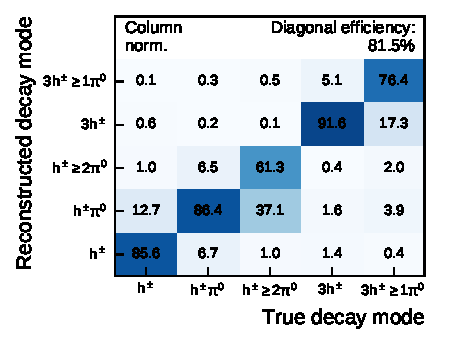
\includegraphics{./figures/decay_mode_classification/combined_sub_e_moments_shots_conv_ptcut_1_5/mig_mat.pdf}
    \subcaption{Migration matrix}
  \end{subfigure}\hfill
  \begin{subfigure}{0.48\textwidth}
    \centering
    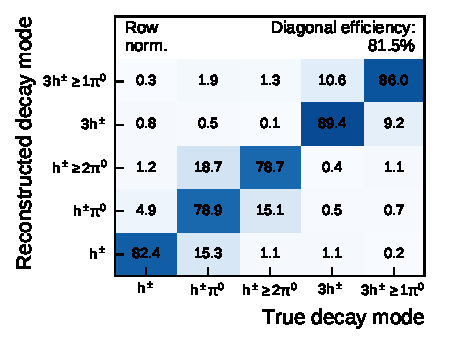
\includegraphics{./figures/decay_mode_classification/combined_sub_e_moments_shots_conv_ptcut_1_5/comp_mat.pdf}
    \subcaption{Purity matrix}
  \end{subfigure}
  \caption{Migration and purity matrices for the extended model including
    conversion, shot and additional cluster information. }
  \label{fig:decay_mode_combined}
\end{figure}

After extending the baseline model, the peaks in the mode probabilities for tau
decays without reconstructed neutral PFOs (cf.\
Figure~\ref{fig:mode_proba_ptcut}) are significantly reduced as the additional
conversion track and shot information can aid in the discrimination even when no
neutral PFOs are present. For completeness the five mode probabilities of the
extended model are summarised in Appendix~\ref{app:combined_probabilities}.

\begin{figure}[htb]
  \begin{subfigure}{0.48\textwidth}
    \centering
    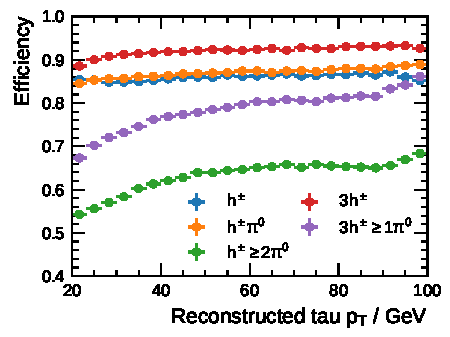
\includegraphics{./figures/decay_mode_classification/combined_sub_e_moments_shots_conv_ptcut_1_5/efficiency_profile.pdf}
    \subcaption{Efficiency profile}
  \end{subfigure}\hfill
  \begin{subfigure}{0.48\textwidth}
    \centering
    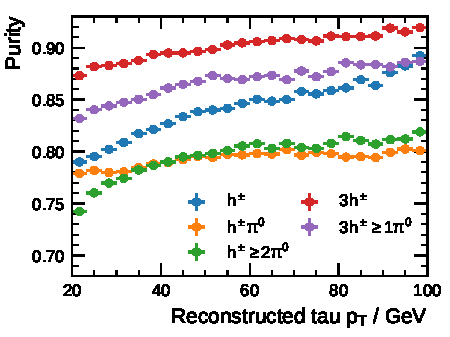
\includegraphics{./figures/decay_mode_classification/combined_sub_e_moments_shots_conv_ptcut_1_5/purity_profile.pdf}
    \subcaption{Purity profile}
  \end{subfigure}
  \caption{Efficiency and purity of the decay mode classification using the
    combined model as a function of reconstructed visible momentum~$p_\text{T}$
    of the tau decay. Evaluated on an independent testing sample.}
  \label{fig:mode_efficiency_purity}
\end{figure}

In Figure~\ref{fig:decay_mode_combined} the migration and purity matrix of the
extended model is shown. The additional discrimination power increases the
diagonal efficiency from \SI{78.0}{\percent} of the baseline model to
\SI{81.5}{\percent}. This is due to an absolute increase in efficiency of the
order of \SI{5}{\percent} for modes containing one or more neutrals
$h^\pm \pi^0$, $h^\pm \geq 2\pi^0$ and $3h^\pm\geq1\pi^0$. The purity is mostly
affected in the $h^\pm$ and $h^\pm \geq 2\pi^0$ modes, where the absolute
improvement is approximately \SI{5}{\percent}. The dependency of mode
classification efficiency and purity on the reconstructed transverse momentum of
the tau lepton is shown in Figure~\ref{fig:mode_efficiency_purity}. The
efficiencies of the $h^\pm$, $h^\pm \pi^0$ and $3h^\pm$ modes show no strong
dependence on the transverse momentum of the tau. In contrast to this the
1-prong mode containing more than one and the 3-prong mode with neutral pions
show a significant increase in efficiency in the \num{20} to \SI{40}{\GeV}
range. This is likely due to difficulties in classfying events containing
neutral pions with low transverse momenta \todo{Reason}. The purity
\todo{Continue}.

The plots in Figure~\ref{fig:mode_efficiency_purity} indicate that the the
RNN-based classification algorithm could be used beyond the design limit of
\SI{100}{\GeV} of the particle flow algorithm, as the efficiencies and purities
remain flat at large transverse momenta. In
Figure~\ref{fig:mode_efficiency_purity_highpt} efficiencies and purities are
shown after retraining the extended model on training data without applying the
upper bound of \SI{100}{\GeV} in reconstructed transverse momentum of the tau.

Diagonal efficiency of \SI{77.6}{\percent} for candidates over \SI{100}{\GeV}.
Wide 'maximum' around \SI{100}{\GeV}. Efficiency flat for most modes except 1pXn
(merging). Purity of modes containing neutrals decreasing. Still fairly large
efficiencies and purities for decays up to \SI{250}{\GeV}ish.

\begin{figure}[htb]
  \begin{subfigure}{0.48\textwidth}
    \centering
    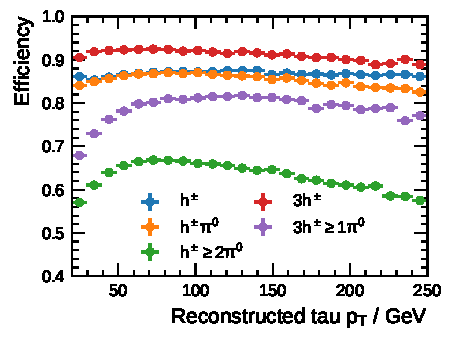
\includegraphics{./figures/decay_mode_classification/highpt/efficiency_profile.pdf}
    \subcaption{Efficiency profile}
  \end{subfigure}\hfill
  \begin{subfigure}{0.48\textwidth}
    \centering
    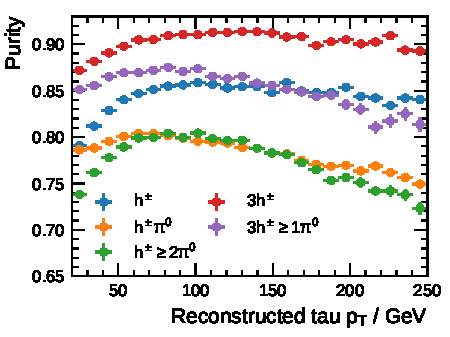
\includegraphics{./figures/decay_mode_classification/highpt/purity_profile.pdf}
    \subcaption{Purity profile}
  \end{subfigure}
  \caption{$p_\text{T}$-dependence of mode efficiency and purity. Retraining
    model without upper bound in transverse momentum.}
  \todo[inline]{Larger pt range would be useful? To show sharp drop.}
  \label{fig:mode_efficiency_purity_highpt}
\end{figure}

The improvements in overall classification power can be employed in
$\mathcal{CP}$ measurements of the Higgs boson using various decay modes of the
tau lepton~\cite{Berge2014}. An example is
the~$\tau \to \rho + \nu_\tau \to \pi + \pi^0 + \nu_\tau$ decay
for~$H \to \tau\tau$ events corresponding to the $h^\pm \pi^0$ mode. This
measurement requires the neutral pions to be reconstructed and identified in the
measured final state. The RNN uses global features of the tau decay and
therefore does not provide a set of neutral PFOs responsible for the decision.
To measure the $\mathcal{CP}$ properties of the Higgs boson an additional
algorithm would be required to identifiy and reconstruct neutral pions given the
classification. For the measurement in the $\rho\nu$ mode using the extended RNN
an absolute improvement in signal efficiency~\SI{7.2}{\percent} and an
improvement in mode purity of~\SI{8.2}{\percent}. Depending on the performance
of reconstructing the neutral pion this could lead to a significant improvement
of the signal to background ratio. The remaining modes show similar improvements
in mode efficiency and purity with respect to the algorithm currently in use at
ATLAS.

Another potential use of the improved classification performance would be to
employ a decay mode specific energy calibration for the measurement of the tau
visible transverse momentum. This could, without the need to explicitly
reconstruct neutral pions, improve the energy resolution of reconstructed
hadronic tau decays.

% $H \to \tautau \to \rho\rho 2 \nu$
% $H \to \tautau \to \pi\pi 2\nu$

%%% Local Variables:
%%% mode: latex
%%% TeX-master: "mythesis"
%%% End:
